\documentclass[12pt, letterpaper]{article}
\usepackage{graphicx}
\usepackage{booktabs}
\usepackage{float}
\usepackage{geometry}
\usepackage{placeins} 
\usepackage{hyperref}
\usepackage{amsmath}


\title{A study on temporary impact and the Almgren-Chriss model, an optimal order execution strategy}
\author{Chaitanya Agarwal}
\date{31 July 2025}


\begin{document}
\maketitle


\section{Modeling temporary impact $g_t(x)$}

\vspace{-0.3em}

Code at 
\href{https://github.com/Chaim3ra/modeling-temp-impact}{github.com/Chaim3ra/modeling-temp-impact}.


\vspace{1em}

We know, the temporary impact function $g_t(x)$ can be defined as the amount of slippage that occurs if $x$ orders are placed at the current time $t$. To effectively model $g_t(x)$, I analyzed the given MBP-10 snapshots of three companies, namely CoreWeave Inc(CRWV), JFrog Ltd(FROG), and SoundHound AI Inc(SOUN). Each snapshot provides the top ten bid and ask price-size pairs, from which I compute the mid-price $m_t$ and the spread. For each snapshot, I then "walk" the ask book, filling shares at successive price levels until \(x\) shares are filled. Slippage can then be calculated as:

\[g_t(x) \;=\;\frac{1}{x}\sum_{k=1}^{K}\bigl(p_k - m_t\bigr)\,\Delta x_k\]



For my initial simulations, I considered the following order sizes \newline $\{5, 50, 100, 500, 1000\}$ to get a rough sense of the slippage curves. After plotting the median slippage curves on log-log axes(Figure \ref{fig:slippage_fixed_grid}), we observe that for CRWV and FROG, slippage grows with order size. 
However, slippage remains flat for SOUN until larger order sizes($x  \geq 1000$). To capture a more representative curve for SOUN, I used a log-spaced grid of 7 unique points from 50 to 5000 shares(which increased the filesize from 3.38GB to 4.45GB).



\begin{figure}[h!] % 'h' means here
    \centering
    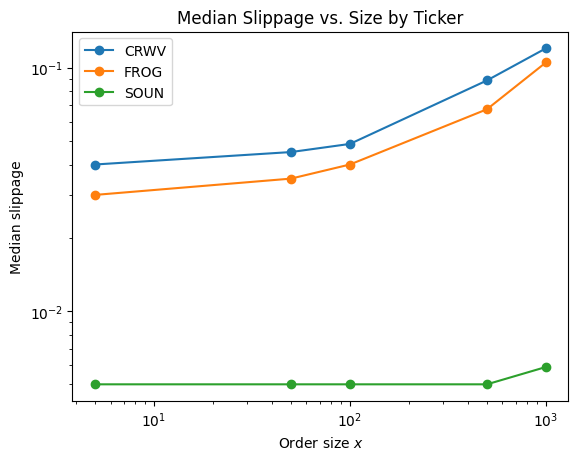
\includegraphics[width=0.6\textwidth]{res/images/median_slippage_small_grid.png} % Adjust width as needed
    \caption{Median Slippage for fixed grid}
    \label{fig:slippage_fixed_grid}
\end{figure}



\begin{figure}[h!] % 'h' means here
    \centering
    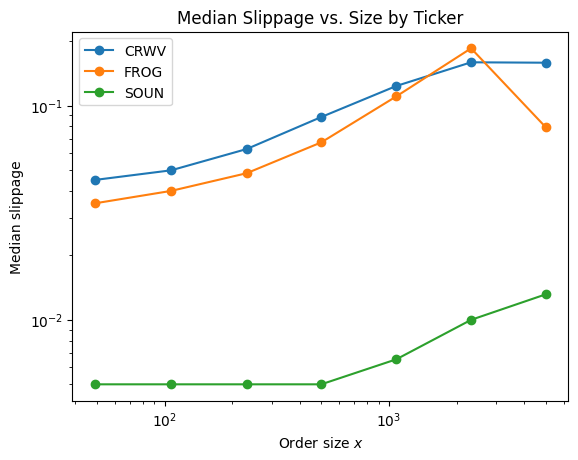
\includegraphics[width=0.6\textwidth]{res/images/median_slippage_med_grid.png} % Adjust width as needed
    \caption{Median Slippage for log-spaced grid}
    \label{fig:slippage_log_grid} 
\end{figure}


The updated median slippage curves(Figure \ref{fig:slippage_log_grid}) now show SOUN rises sharply as the order size increases past 1000. The curves exhibit a concave trend where smaller order sizes incur a very small cost. If the order size was to be doubled, the increase in slippage would be far less than twofold. From my research, this behaviour points us towards two potential models:
\begin{itemize}
    \item \textbf{Linear}: $g(x) = \beta x$, which will serve as my baseline.
    \item \textbf{Power-law}: $g(x) = \alpha x^\gamma$, which exhibits concavity similar to the slippage curves.
\end{itemize}



I fit the aforementioned models to the median slippage data and report the estimated parameters, RMSE, and $R^2$ for the models, proving that power-law fits significantly better than any linear model.

\begin{table}[ht]
\centering
\begin{tabular}{lrrr} 
\toprule
Ticker & $\beta$ & RMSE & $R^2$ \\
\midrule 
CRWV  & $4.30\times10^{-5}$ & $3.407\times10^{-3}$ & $-0.6382$ \\
FROG  & $3.10\times10^{-5}$ & $4.483\times10^{-3}$ & $-0.8701$ \\
SOUN  & $3.00\times10^{-6}$ & $1.400\times10^{-5}$ & $-0.5688$ \\
\bottomrule
\end{tabular}
\caption{Linear fit results.}
\end{table}

\begin{table}[htbp] 
\centering
\begin{tabular}{lrrrr}
\toprule
Ticker & $\alpha$ & $\gamma$ & RMSE & $\mathrm{R}^2$ \\
\midrule
CRWV  & $1.2402\times10^{-2}$ & $0.3144$ & $1.42\times10^{-4}$ & $0.9649$ \\
FROG  & $1.1103\times10^{-2}$ & $0.2940$ & $1.393\times10^{-3}$ & $0.6835$ \\
SOUN  & $1.7750\times10^{-3}$ & $0.2112$ & $2.00\times10^{-6}$ & $0.7733$ \\
\bottomrule
\end{tabular}
\caption{Power-law fit results.}
\end{table}

\FloatBarrier 


Table 1 shows that the linear model fails to accurately predict slippage at small order sizes(negative $R^2$) and comes close only near larger order sizes. On the other hand, from Table 2 we observe that power-law achieves a very high log-log $R^2$ on average for the three tickers, thus proving its ability to effectively capture concave trends as observed in our slippage curves.

In the section below, I will implement the Almgren-Chriss model to formulate an optimal order executing framework to compute $x_i$ that minimizes total expected slippage. 
\section{Order Execution Strategy}

We know, the temporary impact model $g(x)$ tells us the slippage per-share for any given order size $x$. Let's suppose that we have $S$ total amount of orders that need to be filled over $N$ equal trading periods, we need to decide how many shares $x_1, x_2, \ldots, x_N$ to trade in each trading period so as to minimize slippage. That is:

\[
  \min_{x_1,\dots,x_N\ge0}
    \sum_{i=1}^N g(x_i)
  \quad \text{subject to} \quad
    \sum_{i=1}^N x_i = S,
\]


Thus, this is an optimization problem where each $x_i$ represents the shares executed in trading period $i$, with the goal to minimize temporary impact.

To determine how to slice $S$ over $N$ intervals, we use the Almgren-Chriss model. In the optimal execution model, we work with:
\begin{itemize}
    \item How the price moves 
    \item How our trading affects prices, which is our function from the previous section $g(x)$.
\end{itemize}


The Almgren-Chriss model is given by:

\[
  \min_{x_1,\dots,x_N}
    \sum_{i=1}^N g(x_i)
    \;+\;\lambda\,\mathrm{Var}\Bigl[\sum_{i=1}^N x_i\,\tilde p_i\Bigr]
  \quad\text{s.t.}\quad
    \sum_{i=1}^N x_i = S,
\]

where \(\lambda\) is the risk‐aversion parameter and \(\tilde p_i\) are the random price moves.

If we focus only on how our trading affects prices, the problem reduces to:

\[
  \min_{x_1,\ldots,x_N}\;
    \sum_{i=1}^N g(x_i)
  \quad\text{s.t.}\quad
    \sum_{i=1}^N x_i = S.
\]


We can now fit the parameters $\eta$ and $\Gamma$ to the median slippage data, which can then be solved using CVXPY(a convex optimization library in Python) to calculate the optimal shares($x_i$).


\vspace{1em}

Another way to formulate an optimal order executing framework would be to utilize our power-law model from the previous section. That is:
\[\min \sum \alpha x_i^\gamma\]


As this is a concave function, we would need to minimize it using a non-convex solver such as DCCP.




\begin{figure}[h!] % 'h' means here
    \centering
    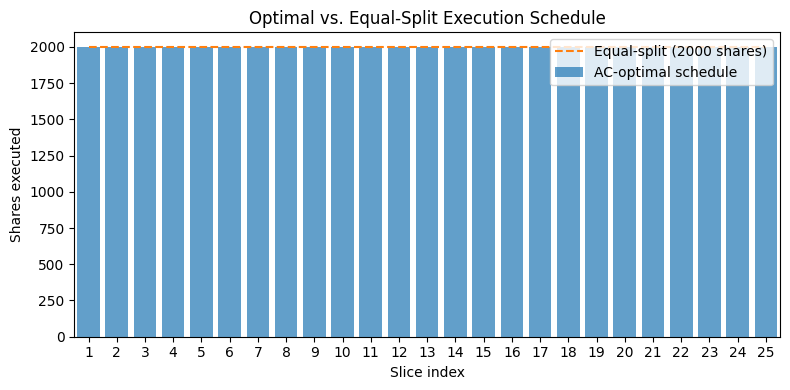
\includegraphics[width=0.79\textwidth]{res/images/optimized_slices_test.png} % Adjust width as needed
    \caption{Optmized slices for S=50,000, N=25}
    \label{fig:optimized_strategy} 
\end{figure}

\end{document}
